%!TEX root = ../../main.tex

Sabe-se que algoritmos de AM necessitam de quantidade significantiva de dados, preferencialmente sem muitos ruídos, para serem utilizados de forma a obter um modelo que possua bom desempenho \cite{marsland}. Levando isto em conta e com vistas a adequar os dados disponíveis com a tarefa de aprendizado considerada, uma etapa de pré-processamento fez-se necessária, cujos passos são descritos a seguir.

Primeiramente foi necessário realizar a adaptação das imagens individuais para as imagens compostas, conforme apresentado anteriormente no esquema da Figura \ref{fig:esquema-solucao}. Para isto, foi feita a combinação de cada assinatura genuína de um autor com suas diferentes versões originais, produzindo uma nova imagem para cada caso, a qual associou-se o rótulo de autêntica. Após esta etapa, também foram combinados os exemplos genuínos com suas respectivas versões forjadas, aos quais foi associado o rótulo de forjado. Todas as imagens obtidas dessas combinações serão utilizadas como exemplos para o processo de treinamento, validação e teste do modelo proposto.

O processo de combinação das imagens de cada um dos exemplos foi realizado em três etapas. Na primeira etapa, ambas as imagens foram redimensionadas para um tamanho de $256 \times 256$ \emph{pixels}. Em seguida, as imagens foram concatenadas verticalmente com a intenção de formar uma única imagem de $256 \times 512$ \emph{pixels}. Por fim, a imagem resultante foi redimensionada novamente em um tamanho de $256 \times 256$ \emph{pixels} e transformada para um espaço de cores em escala de cinza, com a intenção de padronizar todos os exemplos.

% Escrever algo sobre como foi atingida a quantidade de exemplos atual?

Ao concluir a etapa anterior, percebeu-se uma desproporção significativa no número de exemplos de cada classe, o que poderia comprometer o processo de aprendizado do modelo. Para contornar este problema, foram então consideradas três abordagens distintas para os exemplos disponíveis:

\begin{enumerate}
	\item \textbf{Abordagem 1}. Considera apenas os exemplos autênticos para os quais há uma versão forjada. Neste cenário, tem-se apenas $15\%$ de exemplos autênticos e $85\%$ de exemplos forjados;
	\item \textbf{Abordagem 2}. Nesta abordagem foi preservado o total de exemplos autênticos da abordagem anterior, porém o excedente de exemplos forjados que causavam um desbalanceamento evidente foram descartados de maneira pseudo-aleatória. Embora contenha menos exemplos, esta abordagem tem um \emph{dataset} balanceado, com mesma proporção para ambas as classes;
	\item \textbf{Abordagem 3}. Visando um melhor aproveitamento das assinaturas originais no \emph{dataset} NFI, considerou o incremento de assinaturas autênticas, ainda que não haja exemplos forjados para mesma. Obteve-se, então, um \emph{dataset} com mais exemplos e \emph{quasi}-balanceado.  É importante enfatizar que os exemplos forjados desta abordagem são iguais aos da primeira.
\end{enumerate}

Após a organização dos exemplos conforme as abordagens distintas, realizou-se então a partição \emph{holdout} de validação cruzada, com $70\%$ dos exemplos para treinamento, $10\%$ para validação e $20\%$ para testes. A Tabela \ref{tab:divisao-dados} apresenta a descrição destes dados, suas quantidades e divisões e a Figura \ref{fig:divisao-dados} auxilia na visualização da proporcionalidade nas diferentes abordagens consideradas.

\begin{table}[h!]
	\centering
	\caption{Quantitativo de exemplos por abordagem, classe e finalidade na tarefa de aprendizado considerada.}
	\label{tab:divisao-dados}
\resizebox{\textwidth}{!}{
	\begin{tabular}{c c c c c c c c}
		\toprule
		\textbf{Abordagem} & \textbf{Característica} & \textbf{Tipo de Exemplo} & \textbf{Treino} & \textbf{Validação} & \textbf{Teste} & \textbf{Total} & \textbf{Proporção}\\
		\midrule
		\multirow{2}{*}{1} & \multirow{2}{*}{Dados desbalanceados} & Genuíno & 2.011 & 299 & 618 & 2.928 & $15\%$ \\
    &  & Forjado & 11.649 & 1.648 & 3.237 & 16.534 & $85\%$\\
     \midrule
    \multirow{2}{*}{2} & \multirow{2}{*}{Dados balanceados} & Genuíno & 2.011 & 299 & 618 & 2.928 & $50\%$  \\
    &  & Forjado & 2.024 & 308 & 569 & 2.901 & $50\%$ \\
		 \midrule
		\multirow{2}{*}{3} & \multirow{2}{*}{Dados \emph{quasi}-balanceados} & Genuíno & 8.131 & 1.134 & 2.257  & 11.522 & $41\%$\\
		 & & Forjado & 11.649 & 1.648 & 3.237 & 16.534 & $59\%$\\
		\bottomrule
	\end{tabular}}
\end{table}

\begin{figure}[h!]
	\centering
	\caption{Representação gráfica da proporção dos exemplos por abordagem, classe e finalidade na tarefa de aprendizado considerada.}
	\subfloat[Abordagem 1\label{subfig:approach1}]{%
	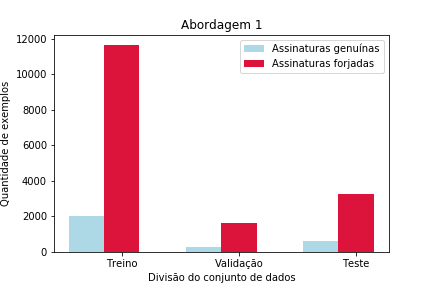
\includegraphics[width=0.5\textwidth]{imgs/approach1}
	}
	\subfloat[Abordagem 2\label{subfig:approach2}]{%
	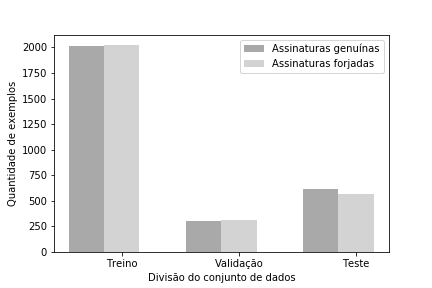
\includegraphics[width=0.5\textwidth]{imgs/approach2}
	}
	\hfill
	\subfloat[Abordagem 3\label{subfig:approach3}]{%
	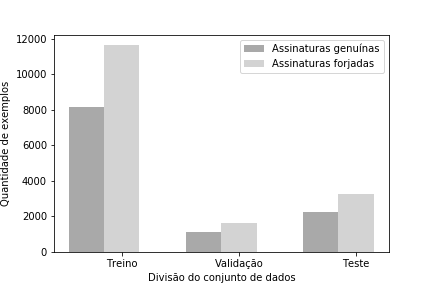
\includegraphics[width=0.5\textwidth]{imgs/approach3}
	}
	\label{fig:divisao-dados}
\end{figure}

Ao serem fornecidas para treinamento pelas CNNs, todos os \emph{pixels} das imagens serão normalizados por meio de uma divisão por $255$, passando a residirem no intervalo $[0,1]$. Esta normalização é realizada em virtude das redes neurais que, em geral, aprendem mais eficientemente nestas condições \cite{chollet}.
